\documentclass[12pt]{article}
\usepackage{graphicx}
\usepackage{amsmath}
\usepackage{multicol}
\usepackage[right=1in,left=1in,top=1in,bottom=1in]{geometry}
\DeclareGraphicsExtensions{.pdf,.png,.jpg,.eps}
\graphicspath{'/Users/Mitch/Dropbox/Adv\ Lab/Lab\ 2/Data/Figures/'}

\begin{document}

\begin{center}
\textbf{Root Finding Techniques and Quantum Wells} \\ 
Mitchell Miller \\
Illinois Institute of Technology \\
January 26 2012 {\ \\ \ \\}
\textbf{Abstract}\\
\end{center}
\noindent
Numerically solving equations is a very common technique used in physical simulations and research.  This lab seeks to explore several different root finding methods ranging from the simple bisection method to the complex hybrid Newton-Raphson technique and apply them to a few quantum well problems.  A brief background into the techniques being studied will be given, followed by a very simple application of each.  Finally, a finite, stepped, and double quantum well will be examined and their solutions presented.
\pagebreak
\section{Introduction}
This lab seeks to study methods for solving a very simple problem:  what value of $x$ causes the result of a given function,  $f(x)$, to be zero?  Often times, this a simple task is easily performed analytically, but, on rare occasion, one's function is especially complicated and difficult to solve via algebra.  In these cases, it is common to use numerical computer methods to derive an answer.  This lab will demonstrate several different techniques ranging from simple to complex, providing an overview of the most common ways of solving for the roots of functions.  
\subsection{Graphical Method}
We begin with the most simple, fastest, and least accurate method of finding a function's root.  This method has one simply plot the function with any graphing utility.  The user then uses the visual representation of the function to approximate the point at which it crosses the x-axis.  The accuracy of the graphical method is extremely limited, and thus it is generally only used as a starting point for the other methods that will be discussed in this lab by providing a range in which one knows the root exists.  
\subsection{Bisection Method}
Progressing towards a more complicated and accurate technique, the bisection method is a very simple way to apply the range that was obtained via the graphical method.  As it is named, this technique works by bisecting the region and testing whether the root is in the left or right section.  
\begin{equation}
\label{midpoint}
x_{mid} = \frac{x_{right}+x_{left}}{2}
\end{equation}
\begin{equation}
\label{bisectionTest}
f(x_{left})*f(x_{mid}) < 0
\end{equation}
If the result of  \eqref{bisectionTest} is true, then the root is found to be in the left half of the initial region and in the right if false.  Using this information, the loop is reinitialized using the new half region as the starting point.  This continues, shrinking the zone in which the root is know to be until reaching a tolerance point, in this case, 8 significant figures.
\begin{equation}
\label{bisectionTol}
|\frac{x_{left}-x_{right}}{x_{mid}}| < 5*10^{-8}
\end{equation}
The tolerance can be varied to any value, but a small tolerance will necessitate a large number of program cycles, increasing computation time.  
\subsection{Newton - Raphson (NR) Method}
The next method to be examined is the NR method.  Instead of beginning with a range of values in which one knows the root exists, this technique requires only a single, rough estimate of the root location and an analytic expression for the derivative of the function.  The algorithm begins at the provided guess, and then calculates the derivative at that point.  It then projects the derivative to the x-axis.  
\begin{equation}
\label{NR1}
x_{n+1} = x_n - \frac{f(x_n)}{\frac{df}{dx}|_{x_n}}
\end{equation}
\begin{equation}
\label{NR2}
f(x) = f(x_0) + (x-x_0)\frac{df}{dx}|_{x_n}
\end{equation}
Although this method seems significantly more difficult than the bisection, the code is quite simple.  Additionally, this technique converges much more quickly than the bisection, decreasing the computational power necessary.
\subsection{Secant Method}
The secant method is a variations of the NR method described above, eliminating the need for an analytic expression for the derivative of the function being solved.  This technique uses the following approximation 
\begin{equation}
\label{derivApprox}
f'(x)\simeq\frac{f(x_i)-f(x_{i-1})}{x_i-x_{i-1}}
\end{equation}
This is the technique that will be used to solve the more complicated quantum applications throughout this lab.
\subsection{Hybrid Method}
The final method for finding function roots presented in this lab is the hybrid method.  This technique is essentially a combination of the NR and bisection methods.  One begins with a left and right point which bound the root.  The left boundary is then used as a starting point for the NR method.  If, at any time, the projection of the function derivative ends up beyond the boundaries, the bisection method is used.  This is determined with the following
\begin{equation}
\label{hybrid}
(x_{left}-x_i)f'(x_i)+f(x_i) < 0 < (x_{right}-x_i)f'(x_i)+f(x_i)
\end{equation}
One then tests the product of the left and right side of \eqref{hybrid}.  If it is less than zero, the NR method continues, and if it is greater, the bisection method is used. 

\section{Applications}
\subsection{Exercises}
There are three different quantum well problems to which the methods discussed above will be applied as well as  two, simple functions to test each method.  The first test function used is given in \eqref{test} while the second function is the eighth Legendre Polynomial, shown in \eqref{legendre}.
\begin{equation}
\label{test}
f(x) = cos(x) - x
\end{equation}
\begin{equation}
\label{legendre}
P_8(x)=\frac{6435x^8-12012x^6+6930x^4-1260x^2+35}{128}
\end{equation}
Considering the simplest equation first, we find the first root of \eqref{test} to be at $x=0.739085$.  Since this is a trigonometric function, there will be repeating roots at higher $x$ values, but those will be ignored.  This root was evaluated with the bisection, NR, and hybrid methods.  Using the bisection method, 26 iterations were necessary, while only 4 were required for the NR method.  

The Legendre polynomial described in \eqref{legendre} has four positive roots.  
\begin{quote}
\begin{center}
1st Root = 0.183435 \\
2nd Root = 0.525532 \\
3rd Root = 0.796666 \\
4th Root = 0.960290 \\
\end{center}
\end{quote}
This set of roots was found using both the hybrid and secant methods.
\subsection{Finite Well}
The first substantial application of the root finding methods discussed above is the problem of a particle in a finite square well.  To solve this problem, we will consider a particle with an energy less than the magnitude of the potential well.
\begin{figure}[!h]
\centering
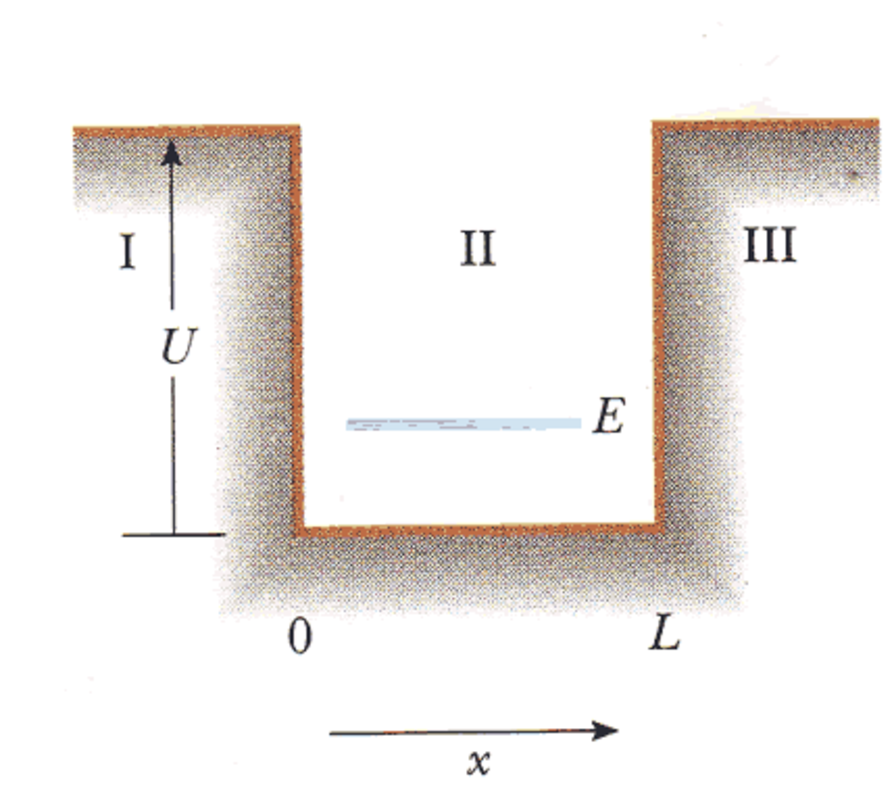
\includegraphics[width =50 mm, height = 50mm]{FiniteWell_diagram.pdf}
\caption{A visual representation of the finite square well.  The well that was evaluated in this lab had parameters U $= 10$ eV and L $=6$ \AA.}
\label{fig:FiniteWellDiagram}
\end{figure}
To solve this in ordinary circumstances the well must be separated into three regions as indicated in \ref{fig:FiniteWellDiagram} and solve the Schrodinger Equation in each of the three regions.
\begin{center}
Region I and III
\end{center}
\begin{equation}
\label{Shro1}
\frac{d^2\psi}{dx^2}-\frac{2m}{\hbar^2}(V_0-E)\psi=0
\end{equation}
\begin{center}
\pagebreak
Region II
\end{center}
\begin{equation}
\label{Shro2}
\frac{d^2\psi}{dx^2}-\frac{2m}{\hbar^2}(E)\psi=0
\end{equation}
The solutions to the Schrodinger Equation in each of these regions are well documented.  For regions I and III, the solution has the form given in \eqref{FiniteWellSoln1}.
\begin{equation}
\label{FiniteWellSoln1}
\psi_I(x)=Ae^{\beta x} , \psi_{III}(x)=Be^{-\beta x} , \text{ where } \beta = \sqrt{\frac{2m(V_0-E)}{\hbar^2}}
\end{equation}
These solutions indicate that there is a non-zero probability that the particle exists in a region that would be forbidden via classical mechanics.  
\begin{equation}
\label{FiniteWellSoln2}
\psi_{II}(x)=C\text{sin}(\alpha x) + D\text{cos}(\alpha x) , \text{ where } \alpha = \sqrt{\frac{2mE}{\hbar^2}}
\end{equation}
The solution for region II is given in \eqref{FiniteWellSoln2}, indicating a bound state within the well.

After determining the wave functions in each of the three regions, one must then determine the energy of each bound state.  By making use of the boundary conditions and a bit of algebra, one can determine an equation for both the even and odd bound states.
\begin{equation}
\label{FiniteWellEven}
\alpha \text{tan}(\alpha a) = \beta \text{ (Even States)}
\end{equation}
\begin{equation}
\label{FiniteWellOdd}
\alpha \text{cot}(\alpha a) = \beta \text{ (Odd States)}
\end{equation}
Using these results as a standard, an alternate method, called the propagator method, can be studied.  A propagator makes use of the known boundary condition of they wave function and its derivative to determine the solution for the entire system.  For a finite well, such as this problem, one begins with the simple solution for the area permitted when using classical mechanics.  At this point, one can easily build a matrix from the unknown coefficients called a propagator matrix.
\[
P_{allowed} =
\left[ {\begin{array}{cc}
\text{cos}[\alpha(x-b)] & \frac{1}{\alpha}\text{sin}[\alpha(x-b)]  \\
 -\alpha \text{sin}[\alpha(x-b)] & \text{cos}[\alpha(x-b)]  \\
\end{array} } \right]
\]
\[
\left[ {\begin{array}{c}
\Psi(x)\\
\Psi'(x) \\
\end{array} } \right] = P_{allowed}
\left[ {\begin{array}{c}
\Psi(b) \\
\Psi'(b)\\
\end{array} } \right]
\]
This matrix 'propagates' the solution from the point $b$ to $x$.  In order to obtain the full solution, this becomes the width of the well.

To solve the problem with the matrix, one begins with the region to the left of the well.  In this region, the solution is known to be an exponential function, give in \eqref{FiniteWellSoln1}.  From this, a relationship between $\Psi(x)$ and $\Psi'(x)$ can be found.
\begin{equation}
\label{DerivRelation1}
\Psi'(x)=\beta\Psi(x),      x < \beta
\end{equation}
A similar relationship can be found for the region to the right of the well.
\begin{equation}
\label{DerivRelation1}
\Psi'(c)=-\beta\Psi(c)
\end{equation}
From this, one can finally arrive at the equation that needs to be solved.
\begin{equation}
\label{PropagatorSolve}
f(E)=\Psi'(c)+\beta\Psi(c)
\end{equation}
Using our matrices from above combined with \eqref{PropagatorSolve}, an analytic expression can be found.  This expression was solved computationally, using the hybrid method.  The results of this equation, as well as the reference results from the standard method are shown in figure \ref{fig:FiniteWell}.
\begin{figure}[!h]
\centering
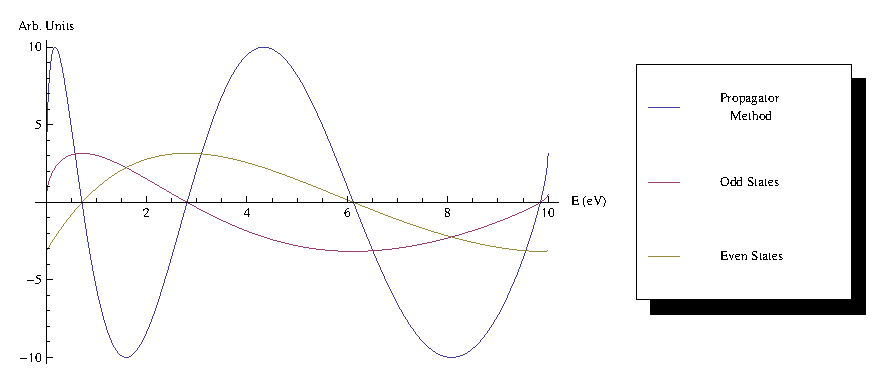
\includegraphics[width =150 mm, height = 80mm]{FiniteWell.pdf}
\caption{An overlay of the two standard solutions (even and odd) to the finite well with the solution obtained via the propagator method.}
\label{fig:FiniteWell}
\end{figure}
From this figure, one can see that roots of the equation obtained via the propagator match perfectly with the even and odd solutions from the standard method.  One important feature to note is the fact that the propagator solution contains both the even and odd states in a single equations.  The roots of this function were found using the hybrid method as the following:
\begin{quote}
\begin{center}
1st Root = 0.760561\\
2nd Root = 2.324734 \\
3rd Root = 6.517475 \\
4th Root = 9.586741 \\
\end{center}
\end{quote}
These roots were confirmed when tested against the standard method.
\subsection{Infinite Stepped Well}
The infinite stepped well is another common problem in quantum mechanics work.  This problem consists of a particle bound to a well of width $a+b$ which has a step of height $V_0$ and width of $b$.  The analytic solution to this system can be found with the same method discussed above:  split the well into to two regions on either side of the step.  At this point, the Schrodinger Equation simplifies greatly, resulting in the same equations found above, \eqref{Shro1} and \eqref{Shro2}.  With these two equations, one obtains a general solution and applies the boundary conditions.  The result will come in the form of two different equations, one for a particle of energy greater than that of the step, \eqref{SteppedGreater}, and one for less,\eqref{SteppedLess}.
\begin{equation}
\label{SteppedGreater}
\beta\text{sin}(\alpha a)\text{cos}(\beta b) + \alpha\text{cos}(\alpha a)\text{sin}(\beta b) = 0 \text{ , where } \beta=\sqrt{\frac{2m(E-V_0)}{\hbar^2}}
\end{equation}
\begin{equation}
\label{SteppedLess}
\beta\text{sin}(\alpha a)\text{cosh}(\beta b) + \alpha\text{cos}(\alpha a)\text{sinh}(\beta b) = 0 \text{ , where } \beta=\sqrt{\frac{2m(V_0-E)}{\hbar^2}}
\end{equation}
The equations are easily solved with numerical methods.  The results of an application of the hybrid method are shown below.

\begin{figure}[!h]
\centering
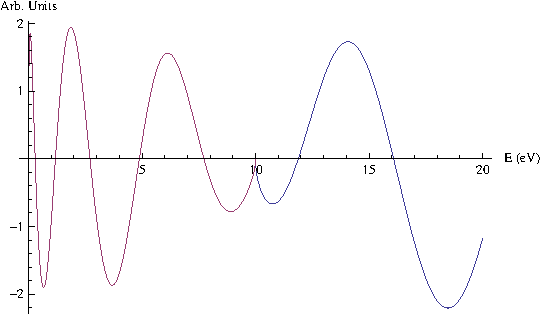
\includegraphics[width =150 mm, height = 80mm]{SteppedWell.pdf}
\caption{The analytic solutions to the stepped well plotted to show a graphical representation of the roots.}
\label{fig:FiniteWellDiagram}
\end{figure}
The discontinuity at 10 eV is a result of the transition from \eqref{SteppedLess} to \eqref{SteppedGreater}.  It is apparent from this figure that there are five bound states for $E < V_0$ and an unlimited number of states fore $E > V_0$.  Using the hybrid method, the roots bound below the step are found to be the following:
\begin{quote}
\begin{center}
1st Root = 0.760561\\
2nd Root = 1.777497\\
3rd Root = 3.605249\\
4th Root = 5.639884\\
5th Root = 8.524289\\
\end{center}
\end{quote}
The first two roots for the states above the potential step were also calculated with the hybrid method.
\begin{quote}
\begin{center}
1st Root = 11.884180\\
2nd Root = 16.084414\\
\end{center}
\end{quote}
The final objective for this problem was to find the minimum well size in which a bound state can exist below the potential step.  This was found using iterations of the hybrid method, decreasing the value of $a$, until no roots exist for \eqref{SteppedLess}.  The results of this program found the minimum value of $a$ to be $1.362$ \AA.  For any $a$ less than this limit, no bound states exist.
\subsection{Double Well}
The final application of the root finding techniques is the double quantum well.  This is an identical system to the singe finite well, however after a short barrier, there is a second well to the right of the first.  From a classical perspective, any particle with energy less than the value of the barrier would be completely confined to its starting well.  However, when quantum mechanics is used, there is a non-zero probability of the particle 'tunneling' through the barrier into the second well.  

This is a quite difficult problem to solve analytically, so it will be convenient to make use of the propagator method outlined above.  The propagator matrix for the allowed region has already been determined, so now the matrix for the region between the two well must be evaluated.  This matrix is again obtained by consider the general solution to a particle in a forbidden barrier and the boundary condition of the system.
\[
P_{forbidden} =
\left[ {\begin{array}{cc}
\text{cosh}[\beta(x-x_0)] & \frac{1}{\beta}\text{sinh}[\beta(x-x_0)]  \\
 \beta \text{sinh}[\beta(x-x_0)] & \text{cosh}[\beta(x-x_0)]  \\
\end{array} } \right]
\]
\[
\left[ {\begin{array}{c}
\Psi(x)\\
\Psi'(x) \\
\end{array} } \right] = P_{allowed}*P_{forbidden}
\left[ {\begin{array}{c}
\Psi(b) \\
\Psi'(b)\\
\end{array} } \right]
\]
For this system, a double well symmetric about the origin, one would propagate $P_{allowed}$ the entire width of the left well and $P_{forbidden}$ through only half of the barrier (from the right edge of the first well to the origin).

The resulting equation obtained from the propagator method can be seen below in figure \ref{fig:DoubleWell}.
\begin{figure}[!h]
\centering
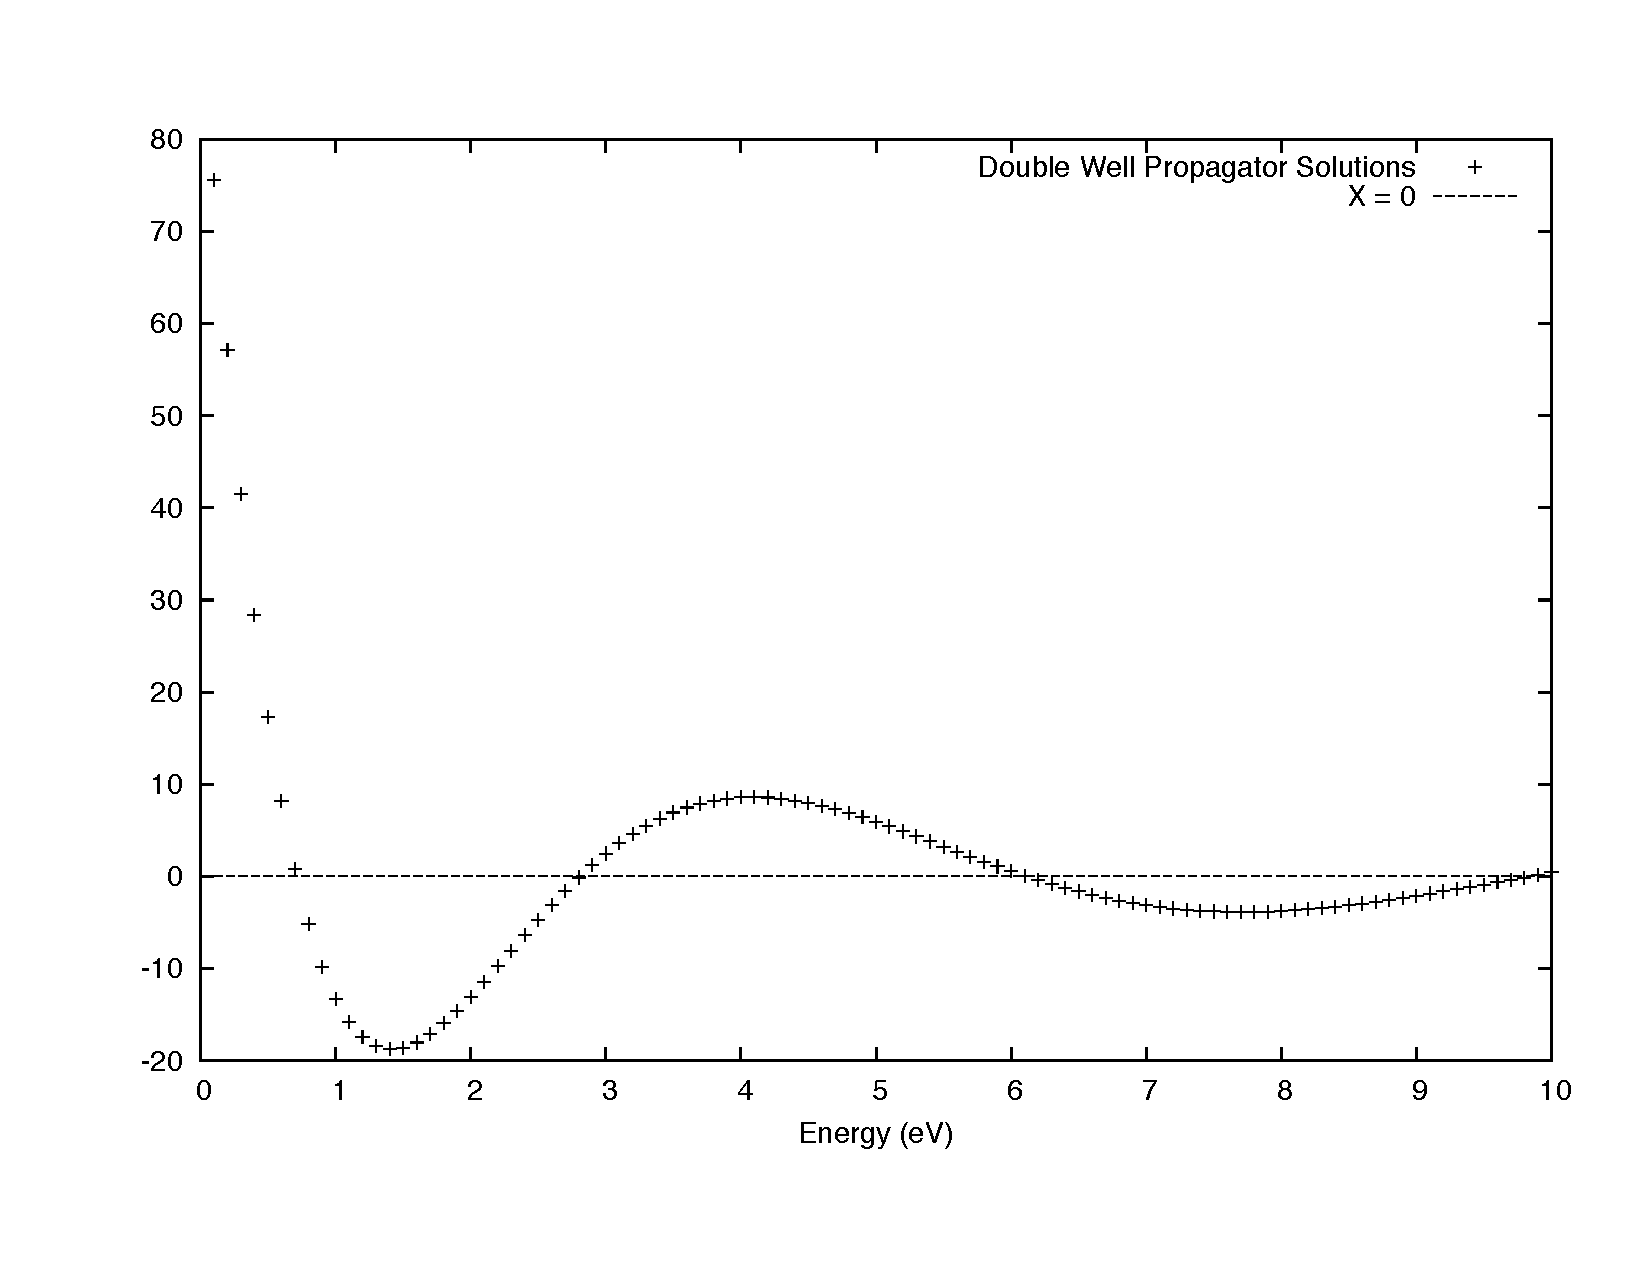
\includegraphics[width =120 mm, height = 65mm]{DoubleWell.pdf}
\caption{Solution to the double well obtained via the propagator method.}
\label{fig:DoubleWell}
\end{figure}
The roots for this problem were, once again, obtained with the hybrid method root finder.  Four bound states were found with the following roots.
\begin{quote}
\begin{center}
1st Root = 0.711807\\
2nd Root = 2.807352\\
3rd Root = 6.120068\\
4th Root = 9.844688\\
\end{center}
\end{quote}
One can also increase the thickness of the barrier to test the results.  When the barrier thickness becomes very large compared to the well width, the system is equivalent to two completely independent finite wells.  This calculation was performed and compared to the results obtained in the previous finite well problem.  The results agree to a very high tolerance.  The final figure shown below depicts several solutions obtained with the propagator method at various barrier thicknesses.
\begin{figure}[!h]
\centering
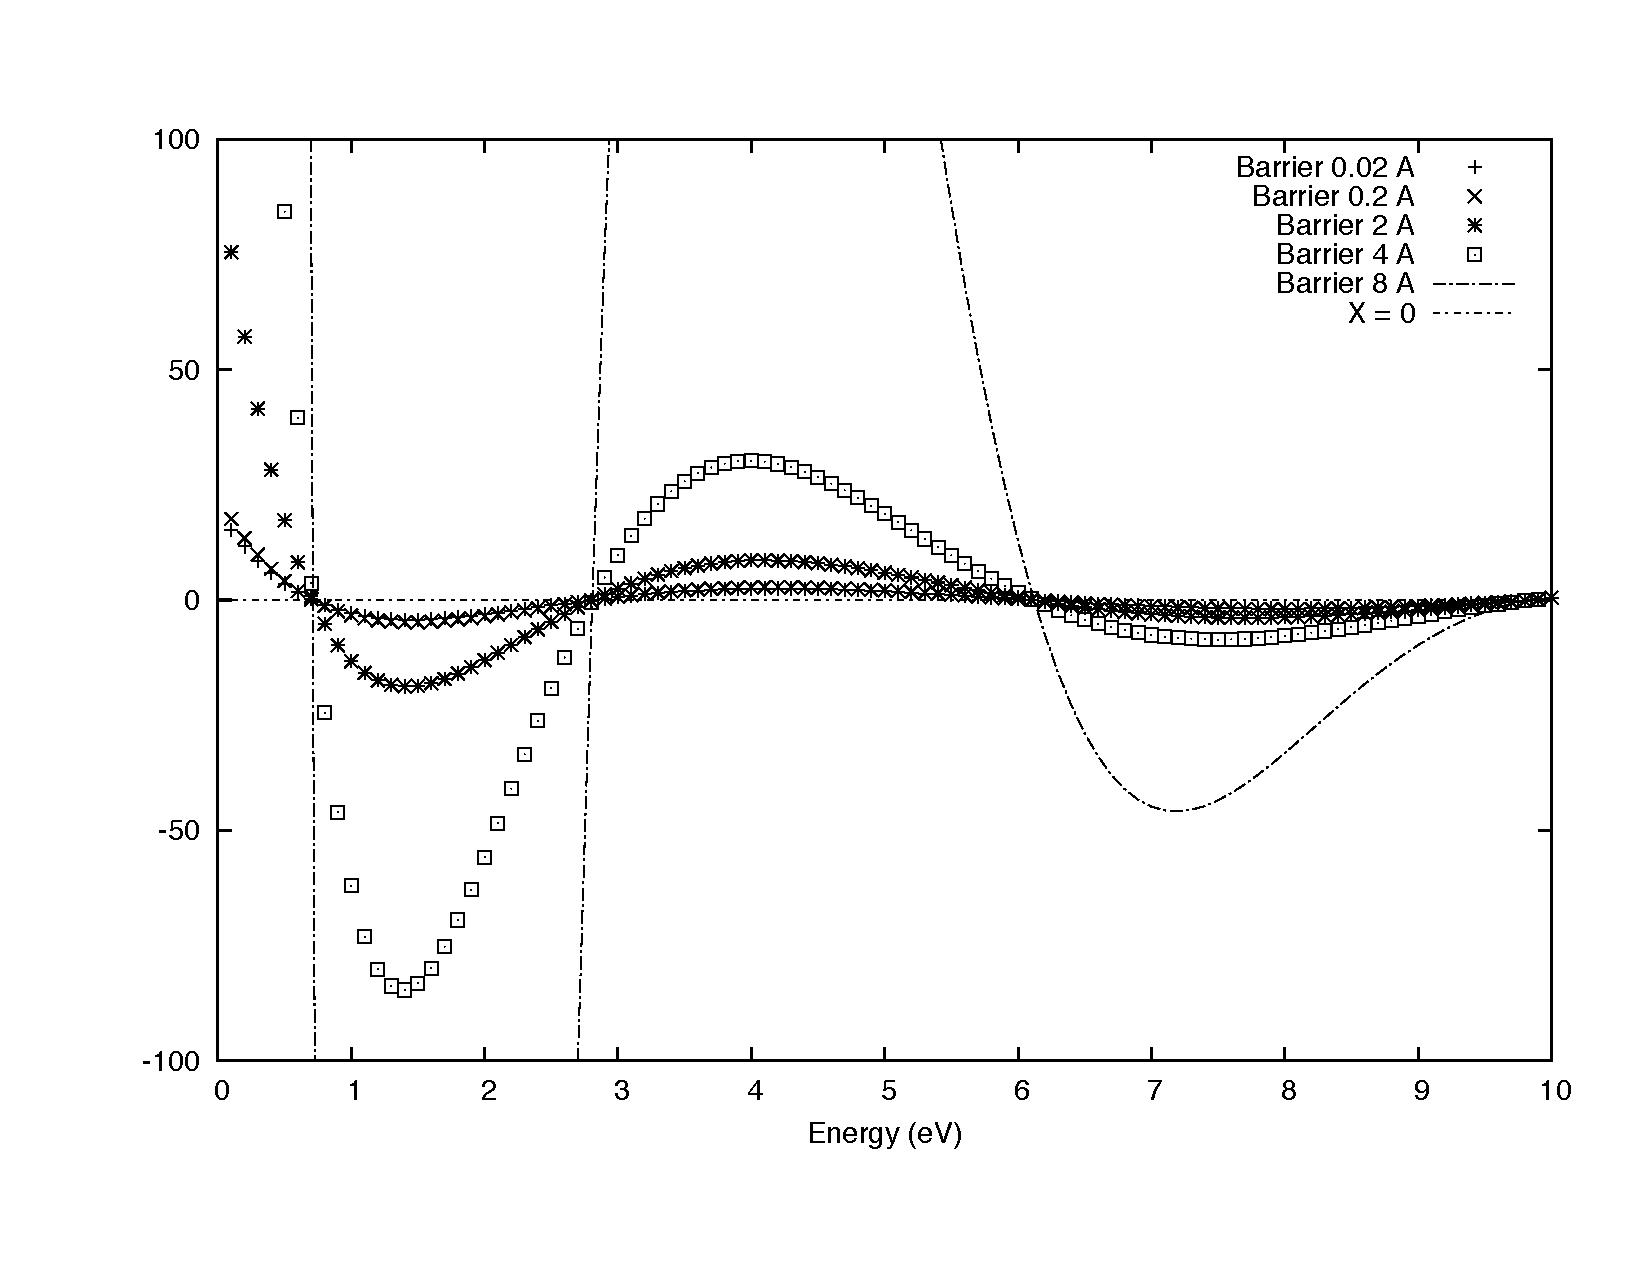
\includegraphics[width =120 mm, height = 80mm]{DoubleWellBarrier.pdf}
\caption{Several different solutions to the double well problem at various barrier thicknesses.}
\label{fig:DoubleWellBarrier}
\end{figure}

\section{Conclusions}
Throughout this lab, several different root finding techniques were discussed.  Each has its own merits but they are all very versatile and incredibly valuable.  Beginning with the simple bisection and progressing through the more complicated Newton Raphson and finally hybrid methods, a few different simple problems were solved.  After establishing the validity of these techniques with simple test equations, more complicated problems were begun.  First, the finite quantum well was examined.  The idea of a propagator matrix was introduced to solve this problem, making later, more difficult problems a much less daunting task.  Next, the stepped, infinite well was presented and the existence of bound states above and below the step explored.  Finally, the double quantum well was solved using the propagator method.  These problems all successfully demonstrated the behavior and capabilities of root finding techniques.


\pagebreak
\section{Code}
\subsection{Exercise 2.1}
\begin{verbatim}
#include <stdio.h>
#include <stdlib.h>
#include <math.h>
#define pi 3.141592654

// Mitchell Miller
// PHYS 440 Lab 1
// Exc. 2.1 1/18/12
// Biseciton Method

double function(double x){

	// Specify desired function
	return(cos(x)-x);

}

int main() {

	// Initialize variables
	double left = 0;
	double right = pi/2;
	double funcLeft, funcRight;
	double mid, funcMid;
	double error;
	double tol = 0.00000005;
	int counter = 0;
	double product;

	funcRight = function(right);
	funcLeft = function(left);
	error = 10*tol;

	while(error > tol){

		mid = (right + left) / 2;
		funcMid = function(mid);
		product = funcLeft * funcMid;
		counter++;
		
		if(product <= 0.0){	// Restricts zero to left half

			right = mid;
			funcRight = funcMid;

		}
		else{			// Restricts zero to right half

			left = mid;
			funcLeft = funcMid;

		}

		error = fabs((right - left)/mid);

		// Print zero and number of loops
		printf("The function zero = %f\n", mid);
		printf("Number of loops = %i\n",counter);
		printf("Error = %e\n", error);

	}

}
\end{verbatim}
\subsection{Exercise 2.4}
\begin{verbatim}
#include <stdio.h>
#include <stdlib.h>
#include <math.h>
#define pi 3.141592654

// Mitchell Miller
// PHYS 440 Lab 1
// Exc. 2.1 1/18/12
// Newton - Raphson Method

double func(double x){

	// Specify desired function
	return(cos(x) - x);

}

double deriv(double x){

	// Provide the derivative of your function
	return(-sin(x) - 1.0);

}

int main() {

	// Initialize variables
	double xValue = 0.8;
	double funcX, derX;
	double delta;
	double error = 1;
	double tol = 0.00000005;
	int counter = 0;

	while(error > tol){

		funcX = func(xValue);
		derX = deriv(xValue);
		delta = (-1) * funcX / derX;
		xValue = xValue + delta;
		error = fabs(delta / xValue);
		counter++;
		
		printf("The function zero = %f\n", xValue);
		printf("Number of loops = %i\n",counter);
		printf("Error = %e\n", error);

	}

}
\end{verbatim}
\subsection{Exercise 2.5}
\begin{verbatim}
#include <stdio.h>
#include <stdlib.h>
#include <math.h>
#define pi 3.141592654

// Mitchell Miller
// PHYS 440 Lab 1
// Exc. 2.1 1/19/12
// Newton - Raphson Method

double func(double x){

	// Specify desired function
	double funcValue;
	funcValue = (1./128.)*(6435.*x*x*x*x*x*x*x*x-12012.*x*x*x*x*x*x+6930.*x*x*x*x-1260.*x*x+35.);
	return(funcValue);

}

double deriv(double x){

	// Provide the derivative of your function
	double derValue;
	derValue = (1./128.)*(6435.*8.*x*x*x*x*x*x*x-12012.*6.*x*x*x*x*x+6930.*4.*x*x*x-1260.*2.*x);
	return(derValue);

}

int main() {

	// Initialize variables
	double xValue = 0.167;
	double funcX, derX;
	double delta;
	double error = 1;
	double tol = 0.00000005;
	int counter = 0;

	while(error > tol){

		funcX = func(xValue);
		derX = deriv(xValue);
		delta = (-1) * funcX / derX;
		xValue = xValue + delta;
		error = fabs(delta / xValue);
		counter++;
		
		printf("The function zero = %f\n", xValue);
		printf("Number of loops = %i\n",counter);
		printf("Error = %e\n", error);

	}

}
\end{verbatim}
\subsection{Exercise 2.8}
\begin{verbatim}
#include <stdio.h>
#include <stdlib.h>
#include <math.h>
#define pi 3.141592654

// Mitchell Miller
// PHYS 440 Lab 1
// Exc. 2.1 1/19/12
// Hybrid Method

double func(double x){

	// Specify desired function
	double funcValue;
	funcValue = x*x-2*x-2;
	return(funcValue);

}

double deriv(double x){

	// Provide the derivative of your function
	double derValue;
	derValue = 2*x-2;
	return(derValue);

}

int main(){

	// Initialize variables
	double left = 0.;
	double right = 3.;
	double fLeft = func(left);
	double fRight = func(right);
	double best, fBest, dBest;
	double funcX, derX;
	double delta;
	int counter;
	double error = 1;
	double tol = 0.00000005;

	if(fabs(fLeft <= fabs(fRight))){

		best = left;
		fBest = fLeft;

	}
	else{

		best = right;
		fBest = fRight;

	}

	dBest = deriv(best);

	while(error > tol){

		counter++;
		if((dBest*(best-left)-fBest) * (dBest*(best-right)-fBest) <= 0){

			delta = -1.*(fBest) / (dBest);
			best = best + delta;

		}
		else{

			delta = (right - left) / 2.0;
			best = (left + right) / 2.0;

		}

		error = fabs(delta / best);

	if(error <= tol){

		printf("The function zero = %f\n", best);

	}
	else{

		fBest = func(best);
		dBest = deriv(best);

		if(fLeft*fBest <= 0){

			right = best;
			fRight = fBest;

		}
		else{

			left = best;
			fLeft = fBest;

		}

	}

	}

}
\end{verbatim}
\subsection{Exercise 2.9}
\begin{verbatim}
#include <stdio.h>
#include <stdlib.h>
#include <math.h>
#define pi 3.141592654

// Mitchell Miller
// PHYS 440 Lab 1
// Exc. 2.1 1/19/12
// Hybrid Method

double func(double x){

	// Specify desired function
	double funcValue;
	funcValue = (1./128.)*(6435.*x*x*x*x*x*x*x*x-12012.*x*x*x*x*x*x+6930.*x*x*x*x-1260.*x*x+35.);
	return(funcValue);

}

double deriv(double x){

	// Provide the derivative of your function
	double derValue;
	derValue = (1./128.)*(6435.*8.*x*x*x*x*x*x*x-12012.*6.*x*x*x*x*x+6930.*4.*x*x*x-1260.*2.*x);
	return(derValue);

}

double hybrid(double left,double right){

	// Initialize variables
	double fLeft = func(left);
	double fRight = func(right);
	double best, fBest, dBest;
	double funcX, derX;
	double delta;
	int counter;
	double error = 1;
	double tol = 0.00000005;

	if(fabs(fLeft <= fabs(fRight))){

		best = left;
		fBest = fLeft;

	}
	else{

		best = right;
		fBest = fRight;

	}

	dBest = deriv(best);

	while(error > tol){

		counter++;
		if((dBest*(best-left)-fBest) * (dBest*(best-right)-fBest) <= 0){

			delta = -1.*(fBest) / (dBest);
			best = best + delta;

		}
		else{

			delta = (right - left) / 2.0;
			best = (left + right) / 2.0;

		}

		error = fabs(delta / best);

		if(error <= tol){

			// printf("The function zero = %f\n", best);

		}
		else{

			fBest = func(best);
			dBest = deriv(best);

			if(fLeft*fBest <= 0){

				right = best;
				fRight = fBest;

			}
			else{

				left = best;
				fLeft = fBest;

			}

		}

	}

	return(best);

}

int main(){

	double rootOne, rootTwo, rootThree, rootFour;
	rootOne = hybrid(0.1,0.3);
	printf("1st Root = %f\n", rootOne);
	rootTwo = hybrid(0.4,0.6);
	printf("2nd Root = %f\n", rootTwo);
	rootThree = hybrid(0.7,0.9);
	printf("3rd Root = %f\n", rootThree);
	rootFour = hybrid(0.95,1.1);
	printf("4th Root = %f\n", rootFour);

}
\end{verbatim}
\subsection{Exercise 2.11}
\begin{verbatim}
#include <stdio.h>
#include <stdlib.h>
#include <math.h>
#define pi 3.141592654

// Mitchell Miller
// PHYS 440 Lab 1
// Exc. 2.1 1/19/12
// Hybrid Method

double func(double x){

	// Specify desired function
	double funcValue;
	funcValue = sin(x) - x/2.;
	return(funcValue);

}

double deriv(double dLeft, double dRight){

	// Provide the approximate derivative of your function
	double derValue;
	derValue = (func(dRight)-func(dLeft))/(dRight-dLeft);
	return(derValue);

}

double hybrid(double left,double right){

	// Initialize variables
	double fLeft = func(left);
	double fRight = func(right);
	double best, fBest, dBest;
	double funcX, derX;
	double delta;
	int counter;
	double error = 1;
	double tol = 0.00000005;

	if(fabs(fLeft <= fabs(fRight))){

		best = left;
		fBest = fLeft;

	}
	else{

		best = right;
		fBest = fRight;

	}

	dBest = deriv(left,right);

	while(error > tol){

		counter++;
		if((dBest*(best-left)-fBest) * (dBest*(best-right)-fBest) <= 0){

			delta = -1.*(fBest) / (dBest);
			best = best + delta;

		}
		else{

			delta = (right - left) / 2.0;
			best = (left + right) / 2.0;

		}

		error = fabs(delta / best);

		if(error <= tol){

			// printf("The function zero = %f\n", best);

		}
		else{

			fBest = func(best);
			dBest = deriv(left,right);

			if(fLeft*fBest <= 0){

				right = best;
				fRight = fBest;

			}
			else{

				left = best;
				fLeft = fBest;

			}

		}

	}

	return(best);

}

int main(){

	double rootOne;
	rootOne = hybrid(pi / 2., pi);
	printf("1st Root = %f\n", rootOne);

}
\end{verbatim}
\subsection{Exercise 2.16 (Finite Well)}
\begin{verbatim}
#include <stdio.h>
#include <stdlib.h>
#include <math.h>
#define pi 3.141592654

// Mitchell Miller
// PHYS 440 Lab 1
// Exc. 2.1 1/19/12
// Hybrid Method

double func(double x){

	// Specify desired function
	double funcValue;
	double c = sqrt(0.2641);
	double v = 10.;
	double a = 6.;
	funcValue = (v-2.0*x)*sin(a*c*sqrt(x))+2.0*x*sqrt(v/x-1.0)*cos(a*c*x);
	return(funcValue);

}

double deriv(double dLeft, double dRight){

	// Provide the approximate derivative of your function
	double derValue;
	derValue = (func(dRight)-func(dLeft))/(dRight-dLeft);
	return(derValue);

}

double hybrid(double left,double right){

	// Initialize variables
	double fLeft = func(left);
	double fRight = func(right);
	double best, fBest, dBest;
	double funcX, derX;
	double delta;
	int counter;
	double error = 1;
	double tol = 0.00000005;

	if(fabs(fLeft <= fabs(fRight))){

		best = left;
		fBest = fLeft;

	}
	else{

		best = right;
		fBest = fRight;

	}

	dBest = deriv(left,right);

	while(error > tol){

		counter++;
		if((dBest*(best-left)-fBest) * (dBest*(best-right)-fBest) <= 0){

			delta = -1.*(fBest) / (dBest);
			best = best + delta;

		}
		else{

			delta = (right - left) / 2.0;
			best = (left + right) / 2.0;

		}

		error = fabs(delta / best);

		if(error <= tol){

			// printf("The function zero = %f\n", best);

		}
		else{

			fBest = func(best);
			dBest = deriv(left,right);

			if(fLeft*fBest <= 0){

				right = best;
				fRight = fBest;

			}
			else{

				left = best;
				fLeft = fBest;

			}

		}

	}

	return(best);

}

int main(){

	double rootOne, rootTwo, rootThree, rootFour;
	rootOne = hybrid(0.5,1.0);
	printf("1st Root = %f\n", rootOne);
	rootTwo = hybrid(2.3,3.0);
	printf("2nd Root = %f\n", rootTwo);
	rootThree = hybrid(5.9,7.3);
	printf("3rd Root = %f\n", rootThree);
	rootFour = hybrid(9.5,10.);
	printf("4th Root = %f\n", rootFour);

}
\end{verbatim}
\subsection{Exercise 2.18 (Double Well)}
\begin{verbatim}
#include <stdio.h>
#include <stdlib.h>
#include <math.h>
#define pi 3.141592654

// Mitchell Miller
// PHYS 440 Lab 1
// Exc. 2.1 1/19/12
// Hybrid Method

double func(double x){

	// Specify desired function
	double funcValue;
	double c = sqrt(0.2641);
	double v = 10.;
	double a = 6.;
	double b = 1.;
	double alpha = c*sqrt(x);
	double beta = c*sqrt(v-x);
	double A,B,C,D;
	double L,M,N,O;
	A=cos(a*alpha);
	B=1./(alpha)*sin(a*alpha);
	C=-1.*alpha*sin(alpha*a);
	D=cos(alpha*a);
	L=cosh(beta*b);
	M=1./beta*sinh(beta*b);
	N=beta*sinh(beta*b);
	O=cosh(beta*b);
	funcValue = C*(L+beta*M)+D*(N+beta*O)+beta*(A*(L+beta*M)+B*(N+beta*O));
	return(funcValue);

}

double deriv(double dLeft, double dRight){

	// Provide the approximate derivative of your function
	double derValue;
	derValue = (func(dRight)-func(dLeft))/(dRight-dLeft);
	return(derValue);

}

double hybrid(double left,double right){

	// Initialize variables
	double fLeft = func(left);
	double fRight = func(right);
	double best, fBest, dBest;
	double funcX, derX;
	double delta;
	int counter;
	double error = 1;
	double tol = 0.00000005;

	if(fabs(fLeft <= fabs(fRight))){

		best = left;
		fBest = fLeft;

	}
	else{

		best = right;
		fBest = fRight;

	}

	dBest = deriv(left,right);

	while(error > tol){

		counter++;
		if((dBest*(best-left)-fBest) * (dBest*(best-right)-fBest) <= 0){

			delta = -1.*(fBest) / (dBest);
			best = best + delta;

		}
		else{

			delta = (right - left) / 2.0;
			best = (left + right) / 2.0;

		}

		error = fabs(delta / best);

		if(error <= tol){

			// printf("The function zero = %f\n", best);

		}
		else{

			fBest = func(best);
			dBest = deriv(left,right);

			if(fLeft*fBest <= 0){

				right = best;
				fRight = fBest;

			}
			else{

				left = best;
				fLeft = fBest;

			}

		}

	}

	return(best);

}

int main(){

	double rootOne, rootTwo, rootThree, rootFour;
	double xValue=0.,yValue;
	int counter=0;
	
	rootOne = hybrid(0.5,1.0);
	printf("1st Root = %f\n", rootOne);
	rootTwo = hybrid(2.3,3.0);
	printf("2nd Root = %f\n", rootTwo);
	rootThree = hybrid(5.9,7.3);
	printf("3rd Root = %f\n", rootThree);
	rootFour = hybrid(9.5,10.);
	printf("4th Root = %f\n", rootFour);

}
\end{verbatim}
\subsection{Stepped Infinite Well}
\begin{verbatim}
#include <stdio.h>
#include <stdlib.h>
#include <math.h>
#define pi 3.141592654

// Mitchell Miller
// PHYS 440 Lab 1
// Exc. 2.1 1/19/12
// Hybrid Method

double func(double x){

	// Specify desired function
	double funcValue;
	double c = sqrt(0.2641);
	double v = 10.;
	double a = 10.;
	double b = 1.;
	funcValue = sqrt(x-v)*sin(a*c*sqrt(x))*cos(b*c*sqrt(x-v))+sqrt(x)*cos(a*c*sqrt(x))*sin(b*c*sqrt(x-v));
	return(funcValue);

}

double deriv(double dLeft, double dRight){

	// Provide the approximate derivative of your function
	double derValue;
	derValue = (func(dRight)-func(dLeft))/(dRight-dLeft);
	return(derValue);

}

double hybrid(double left,double right){

	// Initialize variables
	double fLeft = func(left);
	double fRight = func(right);
	double best, fBest, dBest;
	double funcX, derX;
	double delta;
	int counter;
	double error = 1;
	double tol = 0.00000005;

	if(fabs(fLeft <= fabs(fRight))){

		best = left;
		fBest = fLeft;

	}
	else{

		best = right;
		fBest = fRight;

	}

	dBest = deriv(left,right);

	while(error > tol){

		counter++;
		if((dBest*(best-left)-fBest) * (dBest*(best-right)-fBest) <= 0){

			delta = -1.*(fBest) / (dBest);
			best = best + delta;

		}
		else{

			delta = (right - left) / 2.0;
			best = (left + right) / 2.0;

		}

		error = fabs(delta / best);

		if(error <= tol){

			// printf("The function zero = %f\n", best);

		}
		else{

			fBest = func(best);
			dBest = deriv(left,right);

			if(fLeft*fBest <= 0){

				right = best;
				fRight = fBest;

			}
			else{

				left = best;
				fLeft = fBest;

			}

		}

	}

	return(best);

}

int main(){

	double rootOne, rootTwo;
	rootOne = hybrid(11.5,12.5);
	printf("1st Root = %f\n", rootOne);
	rootTwo = hybrid(15.5,16.5);
	printf("2nd Root = %f\n", rootTwo);

}
\end{verbatim}
\begin{verbatim}
#include <stdio.h>
#include <stdlib.h>
#include <math.h>
#define pi 3.141592654

// Mitchell Miller
// PHYS 440 Lab 1
// Exc. 2.1 1/19/12
// Hybrid Method

double func(double x){

	// Specify desired function
	double funcValue;
	double c = sqrt(0.2641);
	double v = 10.;
	double a = 6.;
	funcValue = (v-2.0*x)*sin(a*c*sqrt(x))+2.0*x*sqrt(v/x-1.0)*cos(a*c*x);
	return(funcValue);

}

double deriv(double dLeft, double dRight){

	// Provide the approximate derivative of your function
	double derValue;
	derValue = (func(dRight)-func(dLeft))/(dRight-dLeft);
	return(derValue);

}

double hybrid(double left,double right){

	// Initialize variables
	double fLeft = func(left);
	double fRight = func(right);
	double best, fBest, dBest;
	double funcX, derX;
	double delta;
	int counter;
	double error = 1;
	double tol = 0.00000005;

	if(fabs(fLeft <= fabs(fRight))){

		best = left;
		fBest = fLeft;

	}
	else{

		best = right;
		fBest = fRight;

	}

	dBest = deriv(left,right);

	while(error > tol){

		counter++;
		if((dBest*(best-left)-fBest) * (dBest*(best-right)-fBest) <= 0){

			delta = -1.*(fBest) / (dBest);
			best = best + delta;

		}
		else{

			delta = (right - left) / 2.0;
			best = (left + right) / 2.0;

		}

		error = fabs(delta / best);

		if(error <= tol){

			// printf("The function zero = %f\n", best);

		}
		else{

			fBest = func(best);
			dBest = deriv(left,right);

			if(fLeft*fBest <= 0){

				right = best;
				fRight = fBest;

			}
			else{

				left = best;
				fLeft = fBest;

			}

		}

	}

	return(best);

}

int main(){

	double rootOne, rootTwo, rootThree, rootFour, rootFive;
	rootOne = hybrid(0.2,1.0);
	printf("1st Root = %f\n", rootOne);
	rootTwo = hybrid(1.0,1.8);
	printf("2nd Root = %f\n", rootTwo);
	rootThree = hybrid(2.5,3.7);
	printf("3rd Root = %f\n", rootThree);
	rootFour = hybrid(5.1,5.9);
	printf("4th Root = %f\n", rootFour);
	rootFive = hybrid(8.0,8.8);
	printf("5th Root = %f\n", rootFive);

}
\end{verbatim}
\begin{verbatim}
#include <stdio.h>
#include <stdlib.h>
#include <math.h>
#define pi 3.141592654

// Mitchell Miller
// PHYS 440 Lab 1
// Exc. 2.1 1/19/12
// Hybrid Method
// Calculate smallest width of 'a' to have a bound state

double func(double x, double a){

	// Specify desired function
	double funcValue;
	double c = sqrt(0.2641);
	double v = 10.;
	funcValue = (v-2.0*x)*sin(a*c*sqrt(x))+2.0*x*sqrt(v/x-1.0)*cos(a*c*x);
	return(funcValue);

}

double deriv(double dLeft, double dRight, double w){

	// Provide the approximate derivative of your function
	double derValue;
	derValue = (func(dRight,w)-func(dLeft,w))/(dRight-dLeft);
	return(derValue);

}

int main(){

	double width = 1.365;
	int index=0;

	while(index < 10){	

		// Initialize variables
		double left = 5.;
		double right = 10.;
		double best=0., fBest=0., dBest=0.;
		double funcX=0., derX=0.;
		double delta=0.;
		double error = 1;
		double tol = 0.00000005;
		double fLeft = func(left, width);
		double fRight = func(right, width);

		if(fabs(fLeft <= fabs(fRight))){

			best = left;
			fBest = fLeft;

		}
		else{

			best = right;
			fBest = fRight;

		}

		dBest = deriv(left,right,width);

		while(error > tol){

			if((dBest*(best-left)-fBest) * (dBest*(best-right)-fBest) <= 0){

				delta = -1.*(fBest) / (dBest);
				best = best + delta;

			}
			else{

				delta = (right - left) / 2.0;
				best = (left + right) / 2.0;

			}

			error = fabs(delta / best);

			if(error <= tol){

				// printf("The function zero = %f\n", best);

			}
			else{

				fBest = func(best,width);
				dBest = deriv(left,right,width);

				if(fLeft*fBest <= 0){

					right = best;
					fRight = fBest;

				}
				else{

					left = best;
					fLeft = fBest;

				}

			}

		}

		printf("Root = %f\n", best);
		printf("Well Size = %f\n", width);
		width = width - 0.001;
		index++;

	}

}
\end{verbatim}



\end{document}

